\documentclass{article}
\usepackage[utf8]{inputenc}
\usepackage[left=1.5cm,right=1.5cm,top=1.5cm,bottom=2cm,a4paper]{geometry}
\usepackage{graphicx}
\usepackage[colorlinks = true, urlcolor = blue]{hyperref}
\usepackage{kotex}

\setlength{\parindent}{0pt}

\title{
    assignment01\\
    \large How to use the utility git
    }
\author{20142052 정연지}
\date{}

\begin{document}

\maketitle

\section{Start a project}

To start a project, you first have to make an on-line repository. Later, make an local repository. And link to repository. If I modify the local repository, and do 'push', then the on-line repository will be changed.

\subsection{Make a on-line repository}

First, log in to github(\href{https://github.com}{https://github.com}). Then you can see the "New repository" button. Click the button.
\begin{center}
    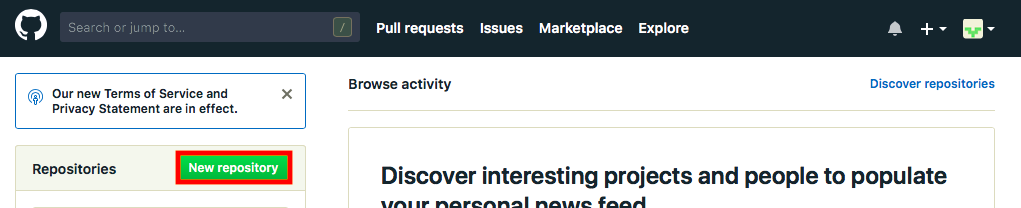
\includegraphics[scale=0.4]{pic/pic1.png}
\end{center}

Then you can create a new repository. Set the repository name, and description.
\begin{center}
    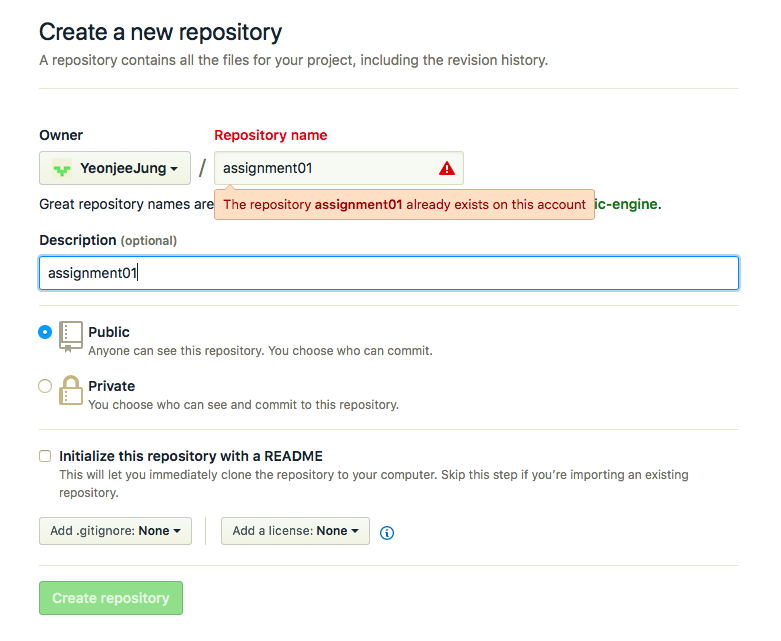
\includegraphics[scale = 0.6]{pic/pic2.png}
\end{center}

\newpage
Now you have an on-line repository!
\begin{center}
    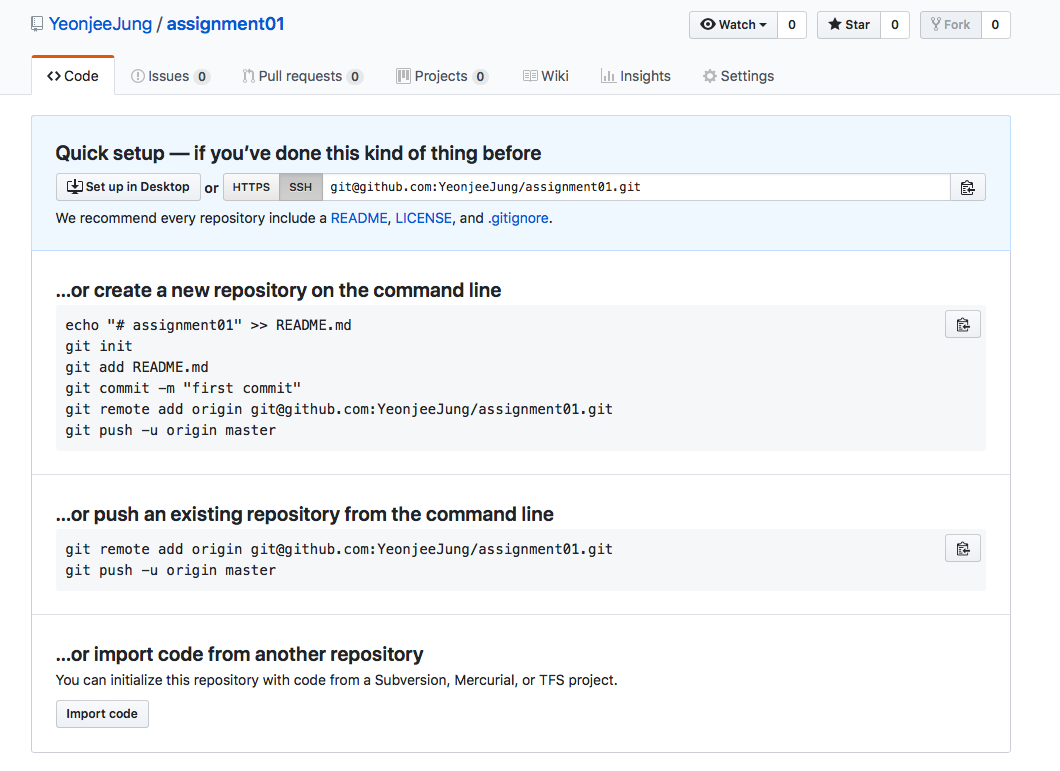
\includegraphics[scale = 0.4]{pic/pic3.png}
\end{center}

The url of my one-line repository is \href{https://github.com/YeonjeeJung/assignment01}{https://github.com/YeonjeeJung/assignment01}

\subsection{Make a local repository}

Return your local computer, make a folder and go into the folder. The folder will be linked with the on-line repository later.
\begin{center}
    
\includegraphics[scale = 0.5]{pic/pic4.png}
\end{center}

Make README.md file. REAME.md is for describing the repository.
\begin{center}
    
\includegraphics[scale = 0.5]{pic/pic5.png}
\end{center}

Initialiaze your local repository. This means you will use this folder for using git.
\begin{center}
    \includegraphics[scale = 0.5]{pic/pic6.png}
\end{center}

Then, add and commit the README.md file. Add means you will capture this moment of the file, and commit means capture this moment of the files that you added. You can do several 'add's before one 'commit'. With '-m' option, you can commit with words.
\begin{center}
    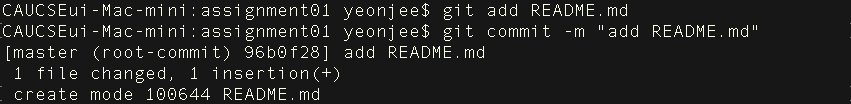
\includegraphics[scale = 0.5]{pic/pic7.png}
\end{center}

\subsection{Link two repositories}
You can use 'git remote add [short name] [url]' command to link your local repository and on-line repository. I used origin as short name.
\begin{center}
    \includegraphics[scale = 0.5]{pic/pic8.png}
\end{center}

\newpage
Now, your two repositories are linked. but in on-line repository, there are no README.md file. You 'push' your commit, then you can see the file in on-line repository.
\begin{center}
    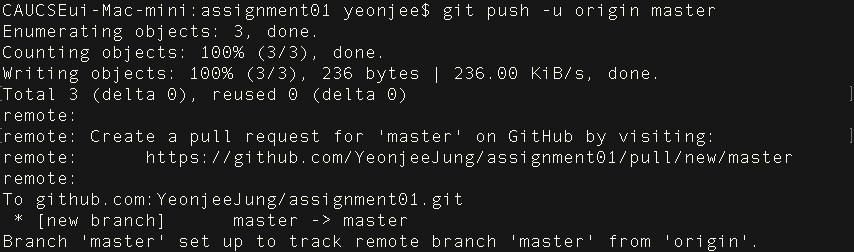
\includegraphics[scale = 0.5]{pic/pic9.png}
\end{center}

Now you can see README.md in on-line repository!
\begin{center}
    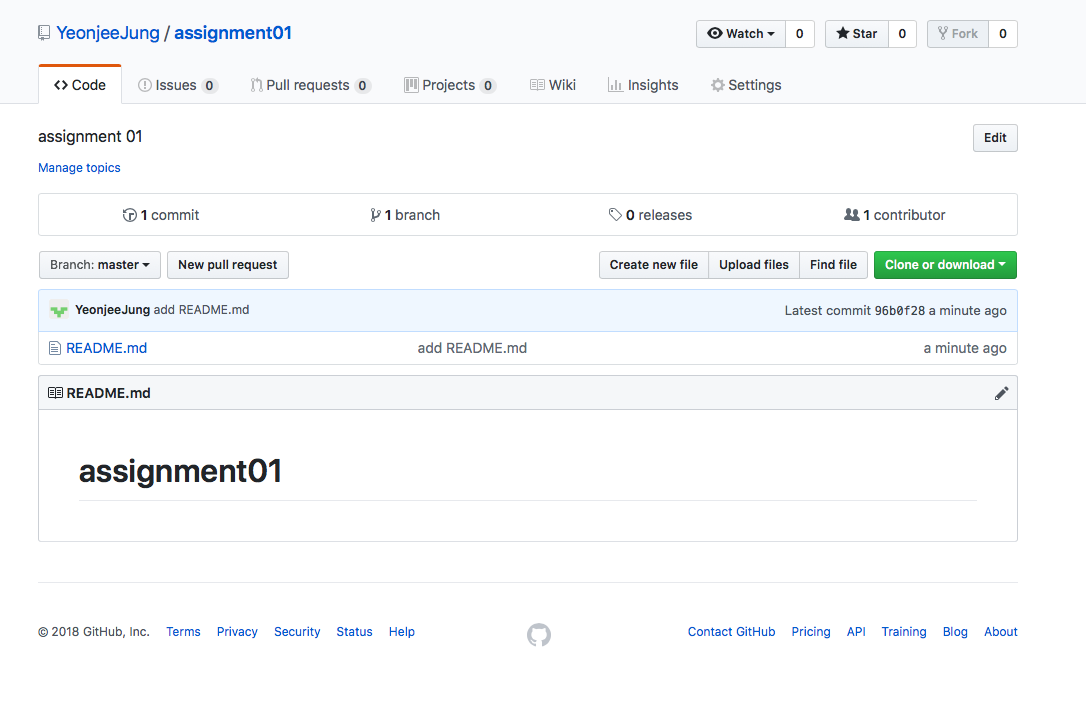
\includegraphics[scale = 0.4]{pic/pic10.png}
\end{center}

\section{Using git in different computers}

The previous works are done in my school computer. And I want to use same things in my laptop, too. So I will link the on-line repository with my laptop, too. In this case, you can use 'clone'. If you already linked two repositories but local repository to update, you can use 'pull'.

\subsection{Clone}

If you do 'clone', git automatically create a directory, link with on-line repository, and copy things in on-line repository. You can see 'assignment01' folder created, and there are things that were in on-line repository.
\begin{center}
    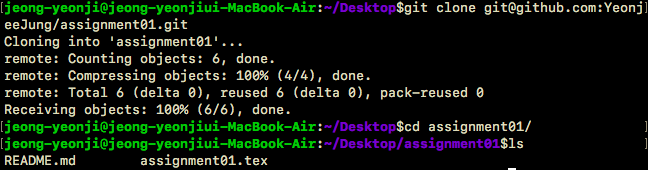
\includegraphics[scale = 0.6]{pic/pic11.png}
\end{center}

\newpage
The folder is already linked, so if you modify, then just do add, commit, push. 'git status' command is for to see the what branch this is, what version this is, and added files.
\begin{center}
    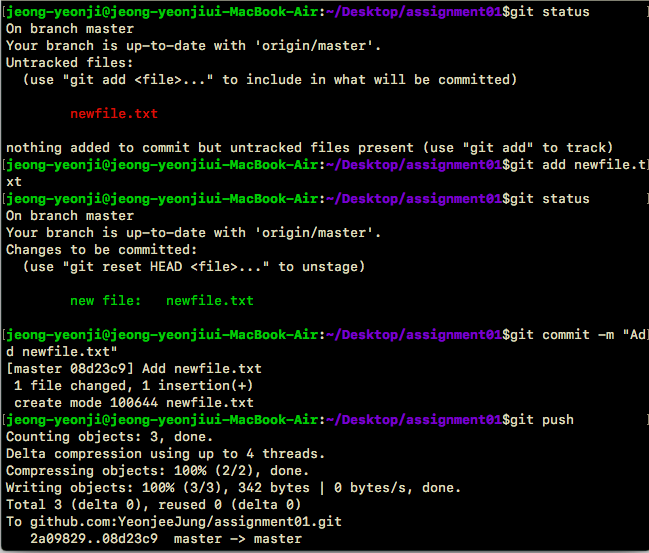
\includegraphics[scale = 0.6]{pic/pic12.png}
\end{center}

\subsection{Pull}

Now, my on-line repository is equal to my home computer. But my school computer is still connected with on-line repository. I want my school computer be same as on-line repository. In this case, you can use 'pull'. Before I do pull, there are no newfile.txt file. After pull, there is the file! That means my school computer updated.
\begin{center}
    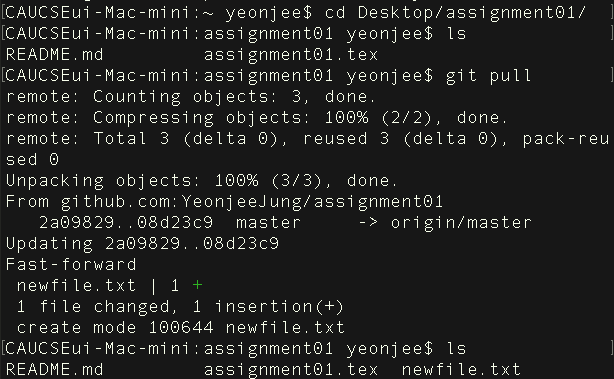
\includegraphics[scale = 0.6]{pic/pic13.png}
\end{center}

\newpage
\section{Version Control}

Git is also good to version control. If you want to go to certain previous commit, you can use 'reset' or 'revert'.

\subsection{Reset : Using --soft option}

If you use --soft option, the head is go back to certain commit, but the file you added are still added and exist in the folder. So, if you just commit, then simply back to the last status. You can see the newfile.txt is still in the folder, and still added.
\begin{center}
    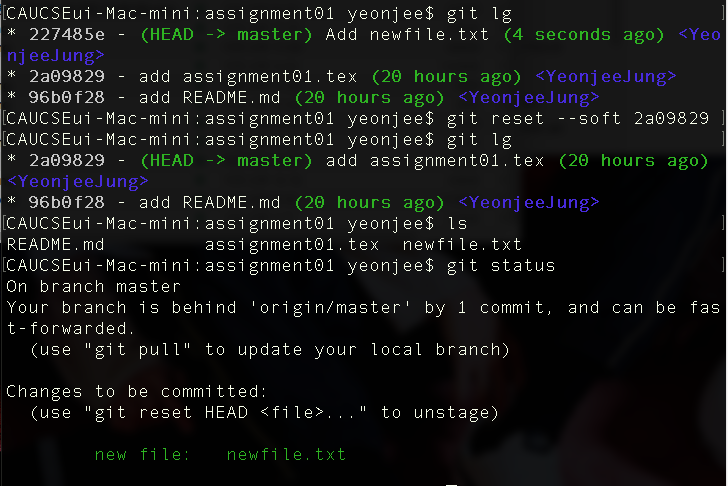
\includegraphics[scale = 0.5]{pic/pic14.png}
\end{center}

\subsection{Reset : Using --mixed option (default)}

If you use --mixed option, the head is go back to certain commit, but the file you added are still exist in the folder. Difference to --soft option is, files that you added are not added this time. You can see newfile.txt is still in ther folder, but is not added.
\begin{center}
    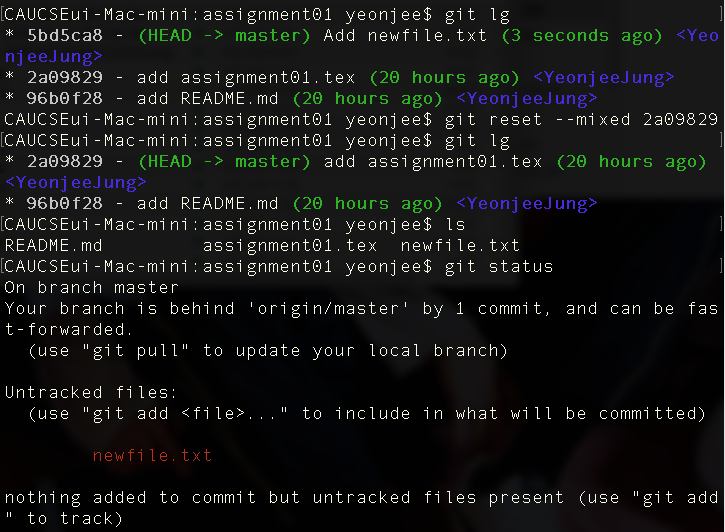
\includegraphics[scale = 0.5]{pic/pic15.png}
\end{center}

\subsection{Reset : Using --hard option}

If you use --hard option, the head is go back to certain commit, and the file you added are not exist. And you cannot go get the file back. So, in using --hard option, you have to seriously concern to do. You cannot see the newfile.txt file this time.
\begin{center}
    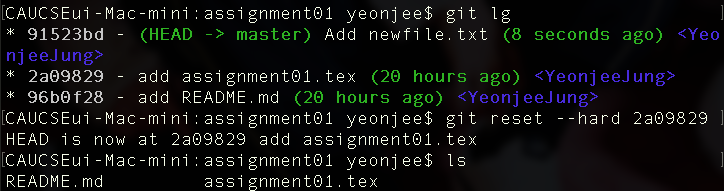
\includegraphics[scale = 0.5]{pic/pic16.png}
\end{center}

\subsection{Revert}

Revert is little different to reset. In reset, the head is go back to commit. But in revert, new commit is created. You can use revert if you want cancel certain commit. You can see the new commit created, and the assignment01.tex file disappeared.
\begin{center}
    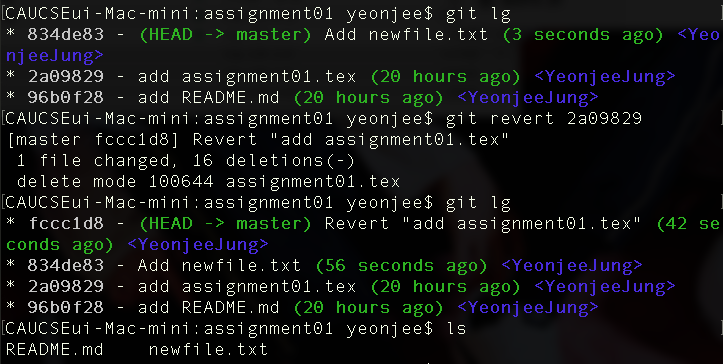
\includegraphics[scale = 0.5]{pic/pic17.png}
\end{center}

\end{document}
